\documentclass[12pt]{article}

\usepackage[margin = .8in]{geometry}
\usepackage{amsmath}
\usepackage{graphicx}
\usepackage{multicol, enumerate, tabularx}

\usepackage{adjustbox}

\usepackage{fancyhdr}
\pagestyle{fancy}

\lhead{Math F113X: Numbers and Society}
\rhead{Date: \hspace{1in}}

\usepackage{tikz}
\usetikzlibrary{calc,trees,positioning,arrows,fit,shapes,through, backgrounds}
\usetikzlibrary{patterns}

\usetikzlibrary{decorations.markings}
\usetikzlibrary{arrows}

\usepackage{pgfplots}

\usepackage{longtable}
\usepackage{tabularx}

\newcommand{\ds}{\displaystyle}
\newcommand{\ans}[1][1in]{\rule{#1}{.5pt}}

\newcommand{\points}[1]{(#1 points.)}		% Trying to be lazy.

\usepackage{array}
\newcolumntype{L}[1]{>{\raggedright\let\newline\\\arraybackslash\hspace{0pt}}m{#1}}
\newcolumntype{C}[1]{>{\centering\let\newline\\\arraybackslash\hspace{0pt}}m{#1}}
\newcolumntype{R}[1]{>{\raggedleft\let\newline\\\arraybackslash\hspace{0pt}}m{#1}}
\newcommand{\red}[1]{\textcolor{red}{#1}}

\newcommand{\be}{\begin{enumerate}}
\newcommand{\ee}{\end{enumerate}}

%\topmargin -1in
%\textheight 9.5in
%\oddsidemargin -0.3in
%\evensidemargin \oddsidemargin
%\pagestyle{empty}
%%\marginparwidth 0.5in
%\textwidth 7in
%\parindent 0in

%--------------------------------------------------------------------------------------------------------------------------------------------------------------------------
%						Document
%--------------------------------------------------------------------------------------------------------------------------------------------------------------------------


\begin{document}
%\pagestyle{fancy}
\begin{center}
{\Large  Worksheet 16 (Scheduling 2): Critical Path Algorithm}
\end{center}



\noindent \textbf{Group Names:} \hrulefill \\
%-------------------------------------------------------------------------------------------------------------
%						Assignment
%-----------------------------------------------------------------------------------------------------
\begin{enumerate}


\item Consider the following digraph:

\newcommand{\mydigraph}{\begin{tikzpicture}[vtx/.style={draw, circle, inner sep = 3pt, font = \scriptsize}, myto/.style={-latex, shorten >=2pt, shorten <=2pt
}, node distance = \r cm]
\node[vtx, label=above:{\scriptsize $T_{1}(10)$}, ] (T1) at (0,0){};
\node[vtx, right =of T1, label=above:{\scriptsize $T_{2}(7)$}] (T2) {};
\node[vtx, right =of T2, label=above:{\scriptsize $T_{3}(4)$}] (T3) {};
\node[vtx, below = \s cm of T1, label=above:{\scriptsize $T_{4}(9)$}] (T4) {};
\node[vtx, right =of T4, label=above left:{\scriptsize $T_{5}(5)$}] (T5) {};
\node[vtx, right =of T5, label= right:{\scriptsize $T_{6}(4)$}] (T6) {};
\node[vtx, below =\s cm of T4, label=below:{\scriptsize $T_{7}(13)$}] (T7) {};
\node[vtx, right =of T7, label=below:{\scriptsize $T_{8}(4)$}] (T8) {};
\node[vtx, right =of T8, label=below:{\scriptsize $T_{9}(6)$}] (T9) {};

\foreach \i/\j in {1/2,2/3,4/5,5/6,7/8,8/9,2/6,5/3,7/5,4/8}{\draw[myto] (T\i) -- (T\j);}
\end{tikzpicture}
}

\def\r{2}
\def\s{.6}
%\begin{center}
\begin{adjustbox}{valign=t,minipage={.4\textwidth}}
\mydigraph
\end{adjustbox}
%\end{center}
%\hspace{1cm}
\begin{adjustbox}{valign=t,minipage={.4\textwidth}}
\begin{tabular}{c | c | c}
time & ready & done \\ \hline
&&\\&&\\&&\\&&\\&&\\&&\\&&\\
\end{tabular}
\end{adjustbox}


\be
\item Use the backflow algorithm to label each vertex in the digraph.

\item Construct a priority list using the Critical Path algorithm. 

\hrulefill

\item Construct a schedule that corresponds to the priority list you just found.

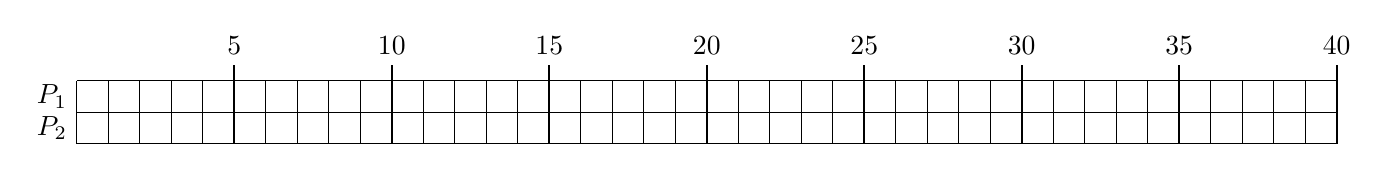
\begin{tikzpicture}[scale = .8]
\path (0, 3/4) node[left] {$P_{1}$};
\path (0, 1/4) node[left] {$P_{2}$};
\draw[step=1/2] (0,0) grid (40/2, 2/2);
\foreach \i in {5, 10, ..., 40}{\draw[thick] (\i/2,0) -- (\i/2,2/2+1/4) node[above]{\i};}
\end{tikzpicture}

\item The schedules that you found on the previous worksheet are shown below:

Priority List $T_{1}, T_{2}, T_{3}, T_{4}, T_{5}, T_{6}, T_{7}, T_{8}, T_{9}$

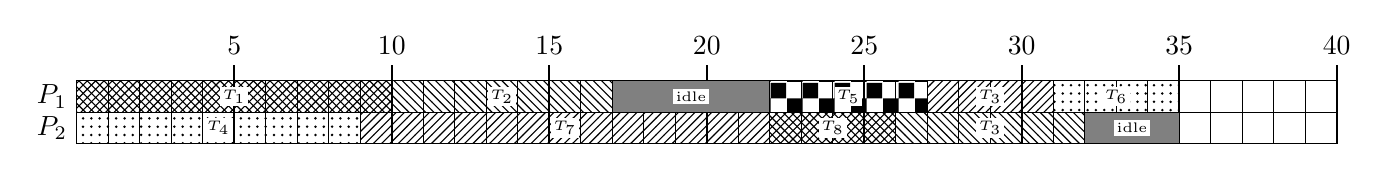
\begin{tikzpicture}[scale = .8, lbl/.style={font=\tiny, inner sep = 1 pt, fill = white}]
\path (0, 3/4) node[left] {$P_{1}$};
\path (0, 1/4) node[left] {$P_{2}$};
\draw[step=1/2] (0,0) grid (40/2, 2/2);
\foreach \i in {5, 10, ..., 40}{\draw[thick] (\i/2,0) -- (\i/2,2/2+1/4) node[above]{\i};}
%processor 1
\filldraw[pattern=crosshatch] (0,1/2) rectangle node[midway, lbl] {$T_{1}$} (10/2,2/2);   
\filldraw[pattern=north west lines,] (10/2,1/2) rectangle node[midway, lbl] {$T_{2}$} (17/2,2/2); 
\filldraw[fill=gray] (17/2,1/2) rectangle node[midway, lbl] {idle} (22/2,2/2);
\filldraw[pattern=checkerboard] (22/2,1/2) rectangle node[midway, lbl] {$T_{5}$} (27/2,2/2); 
\filldraw[pattern=north east lines] (27/2,1/2) rectangle node[midway, lbl] {$T_{3}$} (31/2,2/2); 
\filldraw[pattern=dots] (31/2,1/2) rectangle node[midway, lbl] {$T_{6}$} (35/2,2/2); 
%processor 2
\filldraw[pattern=dots] (0,0) rectangle node[midway, lbl] {$T_{4}$} (9/2,1/2);   
\filldraw[pattern=north east lines,] (9/2,0) rectangle node[midway, lbl] {$T_{7}$} (22/2,1/2); 
%\filldraw[fill=gray] (17/2,0) rectangle node[midway, lbl] {idle} (22/2,1/2);
\filldraw[pattern=crosshatch] (22/2,0) rectangle node[midway, lbl] {$T_{8}$} (26/2,1/2); 
\filldraw[pattern=north west lines] (26/2,0) rectangle node[midway, lbl] {$T_{3}$} (32/2,1/2); 
\filldraw[fill=gray] (32/2,0) rectangle node[midway, lbl] {idle} (35/2,1/2); 
\end{tikzpicture}

Priority list from the Decreasing Time Algorithm: $T_{7}, T_{1}, T_{4}, T_{2}, T_{9}, T_{5}, T_{3}, T_{6}, T_{8}$

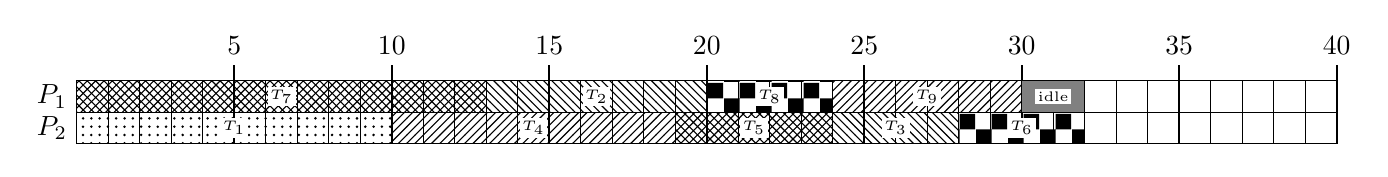
\begin{tikzpicture}[scale = .8, lbl/.style={font=\tiny, inner sep = 1 pt, fill = white}]
\path (0, 3/4) node[left] {$P_{1}$};
\path (0, 1/4) node[left] {$P_{2}$};
\draw[step=1/2] (0,0) grid (40/2, 2/2);
\foreach \i in {5, 10, ..., 40}{\draw[thick] (\i/2,0) -- (\i/2,2/2+1/4) node[above]{\i};}
%processor 1
\filldraw[pattern=crosshatch] (0,1/2) rectangle node[midway, lbl] {$T_{7}$} (13/2,2/2);   
\filldraw[pattern=north west lines,] (13/2,1/2) rectangle node[midway, lbl] {$T_{2}$} (20/2,2/2); 
%\filldraw[fill=gray] (22/2,1/2) rectangle node[midway, lbl] {idle} (24/2,2/2);
\filldraw[pattern=checkerboard] (20/2,1/2) rectangle node[midway, lbl] {$T_{8}$} (24/2,2/2); 
\filldraw[pattern=north east lines] (24/2,1/2) rectangle node[midway, lbl] {$T_{9}$} (30/2,2/2); 
%\filldraw[pattern=dots] (31/2,1/2) rectangle node[midway, lbl] {$T_{6}$} (35/2,2/2); 
\filldraw[fill=gray] (30/2,1/2) rectangle node[midway, lbl] {idle} (32/2,2/2);

%processor 2
\filldraw[pattern=dots] (0,0) rectangle node[midway, lbl] {$T_{1}$} (10/2,1/2);   
\filldraw[pattern=north east lines,] (10/2,0) rectangle node[midway, lbl] {$T_{4}$} (19/2,1/2); 
%\filldraw[fill=gray] (17/2,0) rectangle node[midway, lbl] {idle} (22/2,1/2);
\filldraw[pattern=crosshatch] (19/2,0) rectangle node[midway, lbl] {$T_{5}$} (24/2,1/2); 
\filldraw[pattern=north west lines] (24/2,0) rectangle node[midway, lbl] {$T_{3}$} (28/2,1/2); 
\filldraw[pattern=checkerboard] (28/2,0) rectangle node[midway, lbl] {$T_{6}$} (32/2,1/2); 
\end{tikzpicture}

\item How can you identify the overall critical path given the labels you put on the digraph from the backflow algorithm?
\vfill

\item How does the schedule you found using the critical path priority list compare to the other schedules you found?
\vfill

\ee

\newpage

\def\r{1}

\item Typically the Critical Path algorithm produces a very good schedule, but it may or may not be optimal. Consider the following digraph:
\newcommand{\anotherdigraph}{\begin{tikzpicture}[vtx/.style={draw, circle, inner sep = 3pt, font = \scriptsize}, myto/.style={-latex, shorten >=2pt, shorten <=2pt
}, node distance = \r cm]
\node[vtx, label=above:{\scriptsize $A(10)$}, ] (A) at (0,0){};
\node[vtx, below = \s cm of A, label=above:{\scriptsize $B(5)$}] (B) {};
\node[vtx, below =\s cm of B, label=above:{\scriptsize $F(3)$}] (F) {};
\node[vtx, right = of B, label=above:{\scriptsize $C(4)$}] (C) {};
\node[vtx, right = 2*\r of C, label=above left:{\scriptsize $D(1)$}] (D) {};
\node[vtx, right =of D, label= right:{\scriptsize $E(8)$}] (E) {};
\node[vtx, right = of F, label=below:{\scriptsize $G(1)$}] (G) {};
\node[vtx, right =of G, label=below:{\scriptsize $H(7)$}] (H) {};
\node[vtx, below =\s cm of H, label=below:{\scriptsize $J(6)$}] (J) {};

\foreach \i/\j in {B/C,F/C,F/G,G/H,G/J,C/D,D/E, H/D}{\draw[myto] (\i) -- (\j);}
\end{tikzpicture}
}

\begin{adjustbox}{valign=t,minipage={.4\textwidth}}
\anotherdigraph
\end{adjustbox}
\begin{adjustbox}{valign=t,minipage={.5\textwidth}}
\be
\item Label the graph using the backflow algorithm.

\item Construct the priority list corresponding to the critical path algorithm. 

\hrulefill

\item Construct the priority list corresponding to the decreasing time algorithm. 

\hrulefill

\ee
\end{adjustbox}
%\end{center}
%\hspace{1cm}
%\begin{adjustbox}{valign=t,minipage={.2\textwidth}}
%\begin{tabular}{c | c | c}
%time & ready & done \\ \hline
%&&\\&&\\&&\\&&\\&&\\&&\\&&\\
%\end{tabular}
%\end{adjustbox}
%\begin{adjustbox}{valign=t,minipage={.2\textwidth}}
%\begin{tabular}{c | c | c}
%time & ready & done \\ \hline
%&&\\&&\\&&\\&&\\&&\\&&\\&&\\
%\end{tabular}
%\end{adjustbox}
%\begin{adjustbox}{valign=t,minipage={.2\textwidth}}
%\begin{tabular}{c | c | c}
%time & ready & done \\ \hline
%&&\\&&\\&&\\&&\\&&\\&&\\&&\\
%\end{tabular}
%\end{adjustbox}


%\be
%\item Label the graph using the backflow algorithm.
%
%\item Construct the priority list corresponding to the critical path algorithm. 
%
%\hrulefill

\be

\setcounter{enumii}{3}

\item Construct the schedule using the critical path priority list.

\hspace{-2cm}
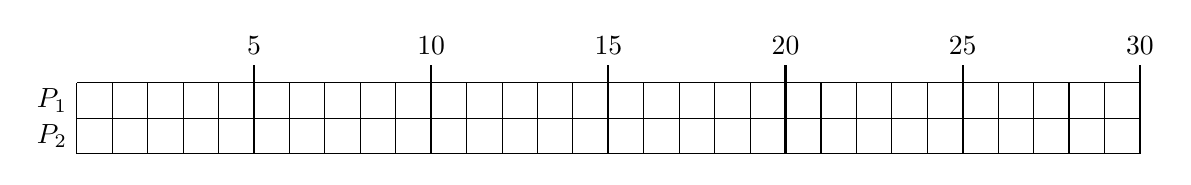
\begin{tikzpicture}[scale = .9, lbl/.style={font=\tiny, inner sep = 1 pt, fill = white}]
\path (0, 3/4) node[left] {$P_{1}$};
\path (0, 1/4) node[left] {$P_{2}$};
\draw[step=1/2] (0,0) grid (30/2, 2/2);
\foreach \i in {5, 10, ..., 30}{\draw[thick] (\i/2,0) -- (\i/2,2/2+1/4) node[above]{\i};}
\end{tikzpicture}
\begin{tabular}{c | c | c}
time & ready & done \\ \hline
&&\\&&\\&&\\&&\\&&\\&&\\&&\\
\end{tabular}

%\item Construct the priority list corresponding to the decreasing time algorithm. 

%\hrulefill



\item Construct the schedule using the decreasing time priority list.

\hspace{-2cm}
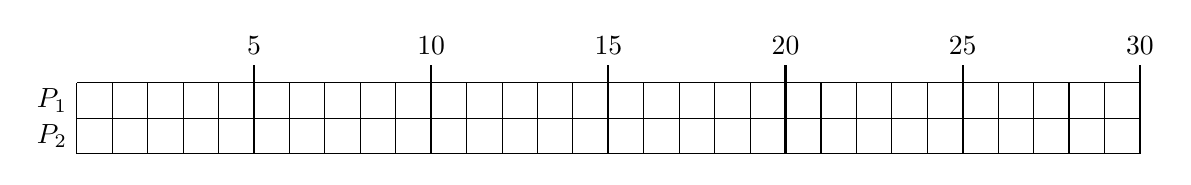
\begin{tikzpicture}[scale = .9, lbl/.style={font=\tiny, inner sep = 1 pt, fill = white}]
\path (0, 3/4) node[left] {$P_{1}$};
\path (0, 1/4) node[left] {$P_{2}$};
\draw[step=1/2] (0,0) grid (30/2, 2/2);
\foreach \i in {5, 10, ..., 30}{\draw[thick] (\i/2,0) -- (\i/2,2/2+1/4) node[above]{\i};}
\end{tikzpicture}
\begin{tabular}{c | c | c}
time & ready & done \\ \hline
&&\\&&\\&&\\&&\\&&\\&&\\&&\\
\end{tabular}

\item \label{goodOne} Construct a schedule using the priority list \[F, B, G, C, H, J, D, A, E\]

\hspace{-2cm}
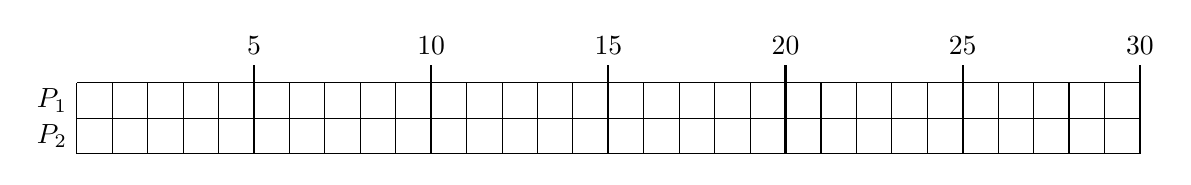
\begin{tikzpicture}[scale = .9, lbl/.style={font=\tiny, inner sep = 1 pt, fill = white}]
\path (0, 3/4) node[left] {$P_{1}$};
\path (0, 1/4) node[left] {$P_{2}$};
\draw[step=1/2] (0,0) grid (30/2, 2/2);
\foreach \i in {5, 10, ..., 30}{\draw[thick] (\i/2,0) -- (\i/2,2/2+1/4) node[above]{\i};}
\end{tikzpicture}
\begin{tabular}{c | c | c}
time & ready & done \\ \hline
&&\\&&\\&&\\&&\\&&\\&&\\&&\\
\end{tabular}

\item How long would it take one processor to complete all the tasks? \ans

\item Explain why the schedule you constructed in (f) must be an optimal schedule for two processors.
\vfil



\ee

%\item For each of the following, circle the correct answer and say a few words.
%
%\begin{enumerate}[{True}  $\quad$ {False} $\quad$ (a)]
%\item The critical path algorithm always produces an optimal schedule.
%\vfill
%\item The decreasing time algorithm always produces a less-optimal schedule than the critical path algorithm.
%\vfill
%\item You can always find an optimal schedule.
%\vfill
%\item Adding more processors will give you a shorter schedule.
%\vfill
%\end{enumerate}


\end{enumerate}
\end{document}

%-------------------------------------------------------------------------------------------------------------------------------------------------------------------------------------------------------------------

%%% Local Variables:
%%% mode: latex
%%% TeX-master: t
%%% End:
